% !TEX encoding = UTF-8
% !TEX TS-program = pdflatex
% !TEX root = ../tesi.tex

%**************************************************************
\chapter{Il progetto di stage}
\label{cap:il progetto di stage}
%**************************************************************

\intro{In questo capitolo, viene descitta la pianificazione e gli obiettivi dello stage. Infine vengono elencati gli strumenti utilizzati durante lo svolgimento dello stage.}\\

%**************************************************************


\section{Pianificazione del lavoro}
\subsection*{Pianificazione settimanale}
\begin{itemize}
    \item Prima Settimana (40 ore)
    \begin{itemize}
        \item Incontro con persone coinvolte nel progetto per discutere i requisiti e le richieste relativamente
        al sistema da sviluppare;
        \item Presentazione strumenti di lavoro per la condivisione del materiale di studio e per la gestione
        dell'avanzamento;
        \item Condivisione scaletta di argomenti;
        \item Ripasso del linguaggio Java SE;
        \item Ripasso concetti Web (Servlet, servizi REST, Json ecc.).
    \end{itemize}
    \item Seconda Settimana (40 ore)
        \begin{itemize}
            \item Studio principi generali di Spring Core (IOC, Dependency Injection);
            \item Studio SpringBoot;
            \item Studio Spring Data/DataRest.
        \end{itemize}
    \item Terza Settimana (40 ore)
        \begin{itemize}
            \item Ripasso linguaggio Javascript;
            \item Studio del linguaggio TypeScript.
        \end{itemize}
    \item Quarta Settimana (40 ore)
        \begin{itemize}
            \item Studio piattaforma NodeJS e AngularCLI;
            \item Studio framework Angular.
        \end{itemize}
    \item Quinta Settimana (40 ore)
        \begin{itemize}
        \item Analisi e studio del progetto SushiLab;
        \item Progettazione ed implementazione della nuova maschera di accesso.
        \end{itemize}
    \item Sesta Settimana (40 ore)
    \begin{itemize}
        \item Progettazione ed implementazione nuova maschera "Inserimento Ordine e gestione del tavolo".
    \end{itemize}
    \item Settima Settimana (40 ore)
    \begin{itemize}
        \item Progettazione ed implementazione nuova maschera "Merge Ordini e Visualizzazione Ordine unico".
    \end{itemize}
    \item Ottava Settimana - Conclusione (40 ore)
    \begin{itemize}
        \item Verifica del funzionamento della web-app;
        \item Validazione della web-app;
        \item Termine integrazioni e collaudo finale.
    \end{itemize}
\end{itemize}

\section{Obiettivi richiesti}
\subsection{Notazione}
Si farà riferimento ai requisiti secondo le seguenti notazioni:
\begin{itemize}
    \item O per i requisiti obbligatori, vincolanti in quanto obiettivo primario richiesto dal committente;
    \item D per i requisiti desiderabili, non vincolanti o strettamente necessari, ma dal riconoscibile valore
    aggiunto;
    \item F per i requisiti facoltativi, rappresentanti valore aggiunto non strettamente competitivo.
\end{itemize}
Le sigle precedentemente indicate saranno seguite da una coppia sequenziale di numeri, identificativo del
requisito.
\subsection{Obiettivi fissati}
Si prevede lo svolgimento dei seguenti obiettivi:
\begin{itemize}
    \item Obbligatori:
    \begin{itemize}
        \item O01: Acquisizione competenze sulle tematiche sopra descritte;
        \item O02: Capacità di raggiungere gli obiettivi richiesti in autonomia seguendo il cronoprogramma;
        \item O03: Portare a termine le implementazioni previste con una percentuale di superamento pari al 80\%.        
    \end{itemize}
    \item Desiderabili:
     \begin{itemize}
        \item D01: Portare a termine le implementazioni previste con una percentuale di superamento pari al 100\%.
     \end{itemize}
     \item Facoltativi:
     \begin{itemize}
        \item F01: Apportare un valore aggiunto al gruppo di lavoro durante le fasi di progettazione delle interfacce.
     \end{itemize}
\end{itemize}


\section{Modalità di lavoro}
L'azienda utilizza lo sviluppo agile del software. La modalità agile aiuta a ridurre il rischio di fallimento sviluppando il software in finestre di tempo limitate chiamate iterazioni che, in genere, durano qualche settimana. Ogni iterazione è un piccolo progetto a sé stante e deve contenere tutto ciò che è necessario per rilasciare un piccolo incremento nelle funzionalità del software: pianificazione, analisi dei requisiti, progettazione, implementazione, test e documentazione. Ogni settimana viene effettuato un incontro con il tutor aziendale per discutere dei problemi trovati durante lo sviluppo e il punto di situazione del progetto.

\section{Strumenti utilizzati}
\subsection{Comunicazione:}
Per avere una buona comunicazione con l'azienda si è deciso di utilizzare:
\subsubsection{Discord:}
Una piattaforma di \gls{voipg}, messaggistica istantanea e distribuzione deigitale. Su discord gli utenti comunicano con chiamate vocali, video chiamate ed è anche possibile condividere lo schermo.
\begin{figure}[H]
    \centering
    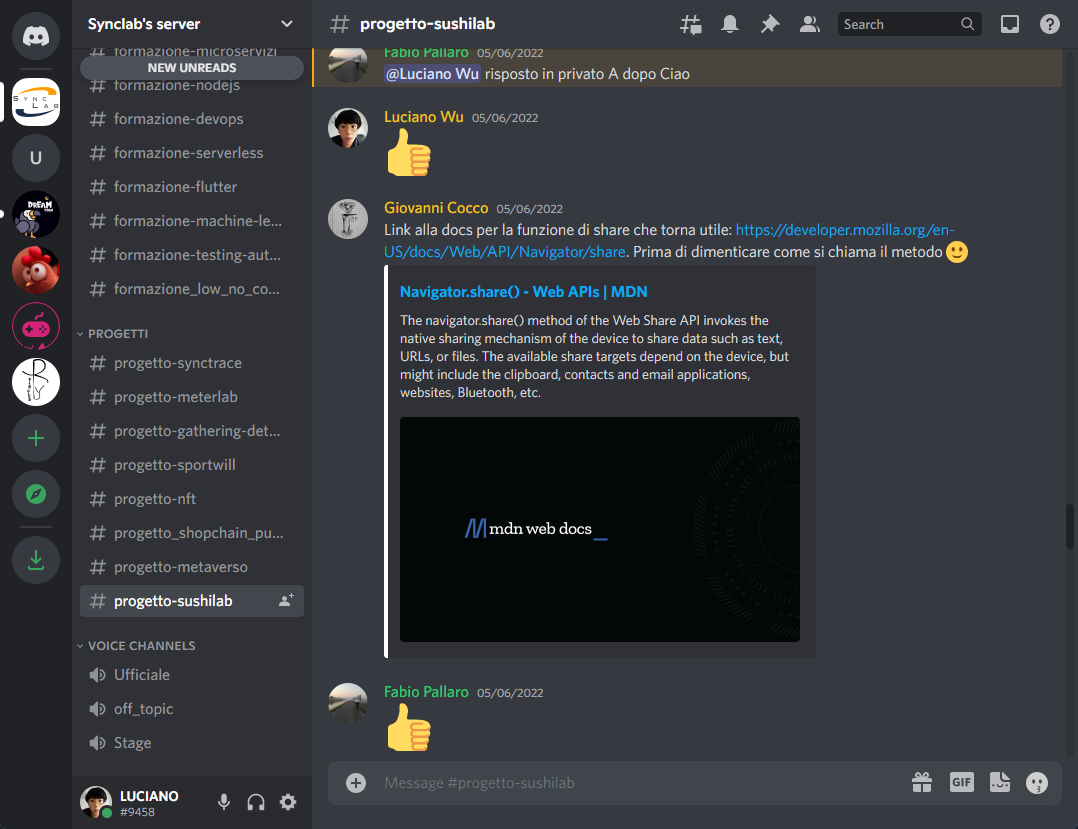
\includegraphics[scale=0.4]{discord.png}
    \caption{Canale SyncLab su Discord}
\end{figure}
\subsubsection{Trello:}
Un software gestionale in stile Kanban, in cui è possibile pianificare il progetto, condividere lo stato di svolgimento di una card con altri collabolatori, spostare vari card tra le liste e assegnare ad un utente.
\begin{figure}[H]
    \centering
    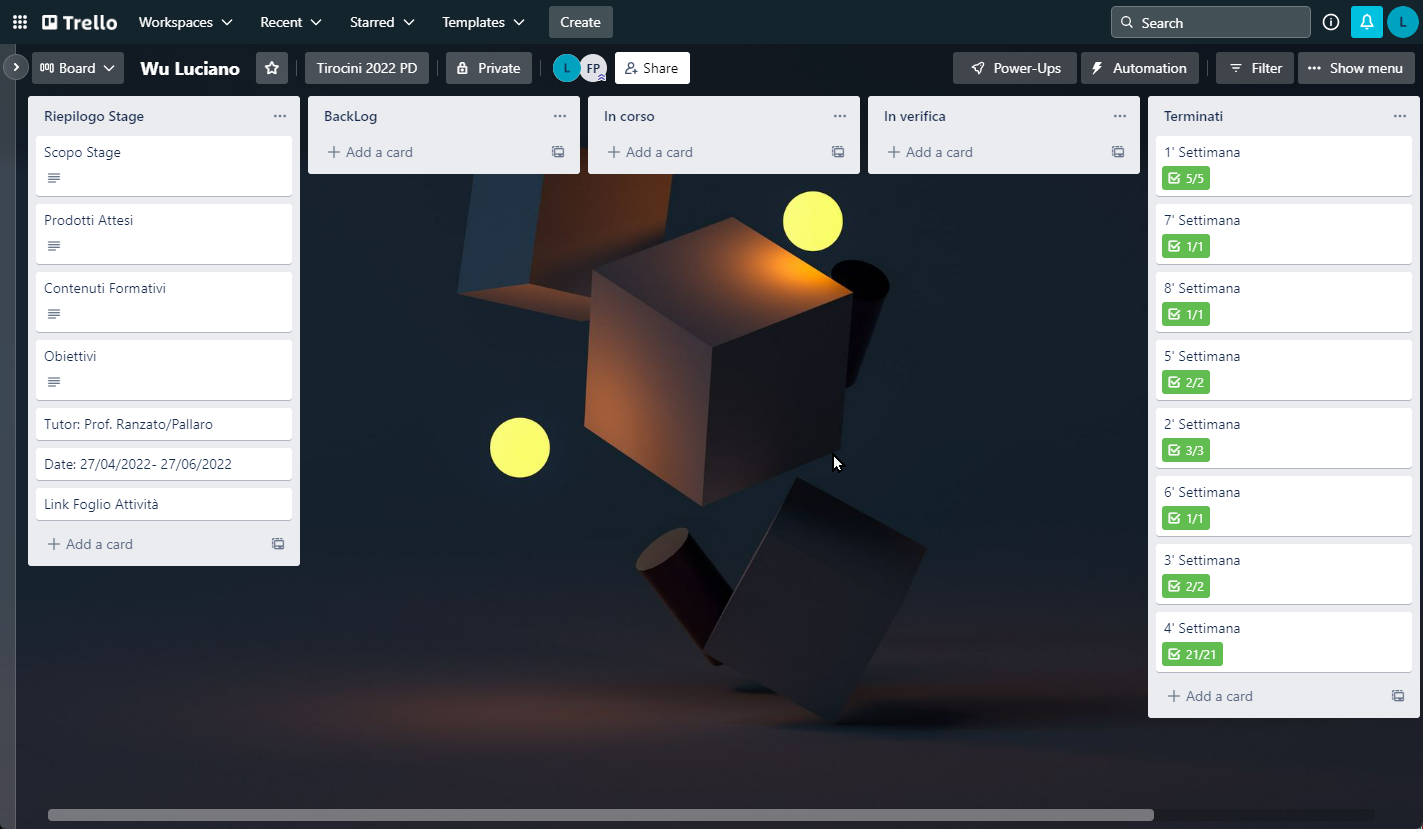
\includegraphics[scale=0.3]{trello.png}
    \caption{Borad di Trello per il progetto sushi-lab}
\end{figure}
\subsubsection{Google Sheets:}
Una web-app che fornisce tutte le funzionalità di un foglio elettronico, lo abbiamo utilizzato come un diario giornaliero, dove vengono descritti il compito svolto durante una certa giornata.
\begin{figure}[H]
    \centering
    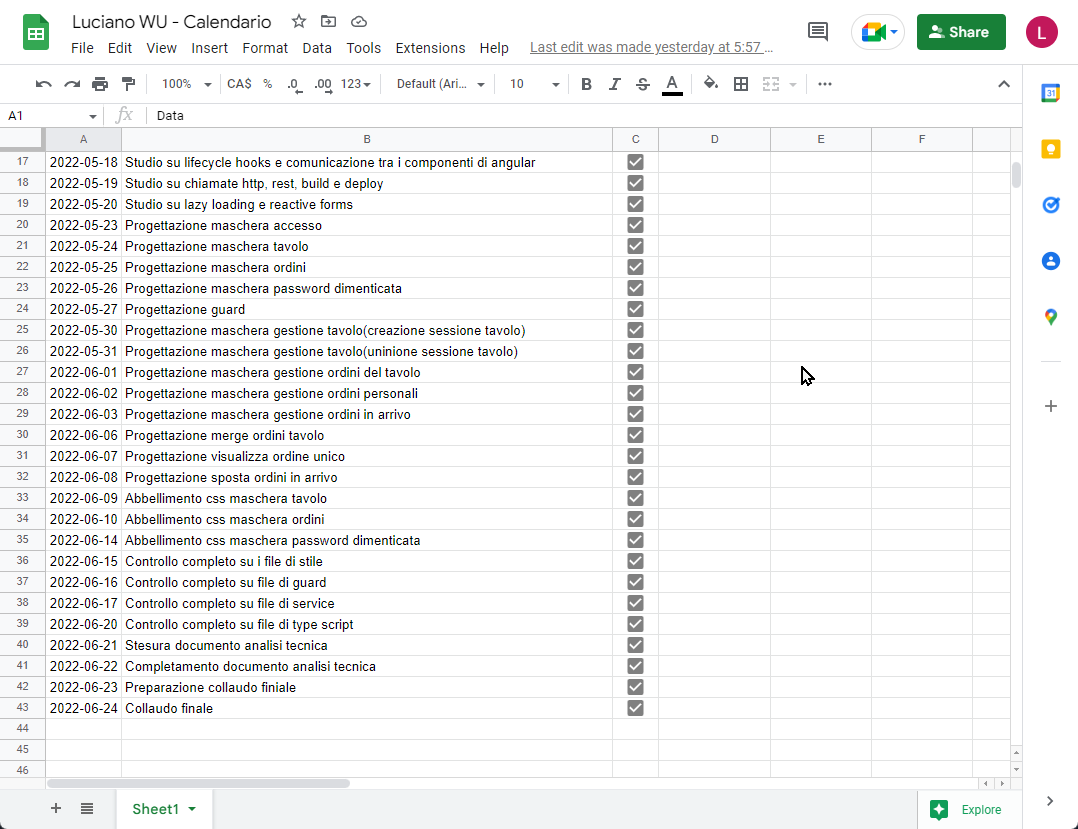
\includegraphics[scale=0.45]{googlesheet.png}
    \caption{Calendario personale per il progetto sushi-lab}
\end{figure}
\subsubsection{Google Meet:}
Un software nato per le videochiamate sviluppato da Google, in cui è possibile mandare messaggi e condividere lo schermo e video contemporaneamente, lo abbiamo utilizzato per alcuni incontri con alcuni collabolatori esterni per analisi dei requisiti.
\subsection{Sviluppo:}
Per avere una buona efficienza per lo sviluppo della web-app vengono utilizzati i strumenti più popolari per lo sviluppo, che sono:
\subsubsection{GitHub:}
Servizio di hosting per il sviluppo software, è implementato insieme con lo strumento di controllo di versione distribuito \gls{Gitg}, nel mio caso è stato utilizzato per condividere e tracciare i file con gli altri collabolatori del progetto.
\begin{figure}[H]
    \centering
    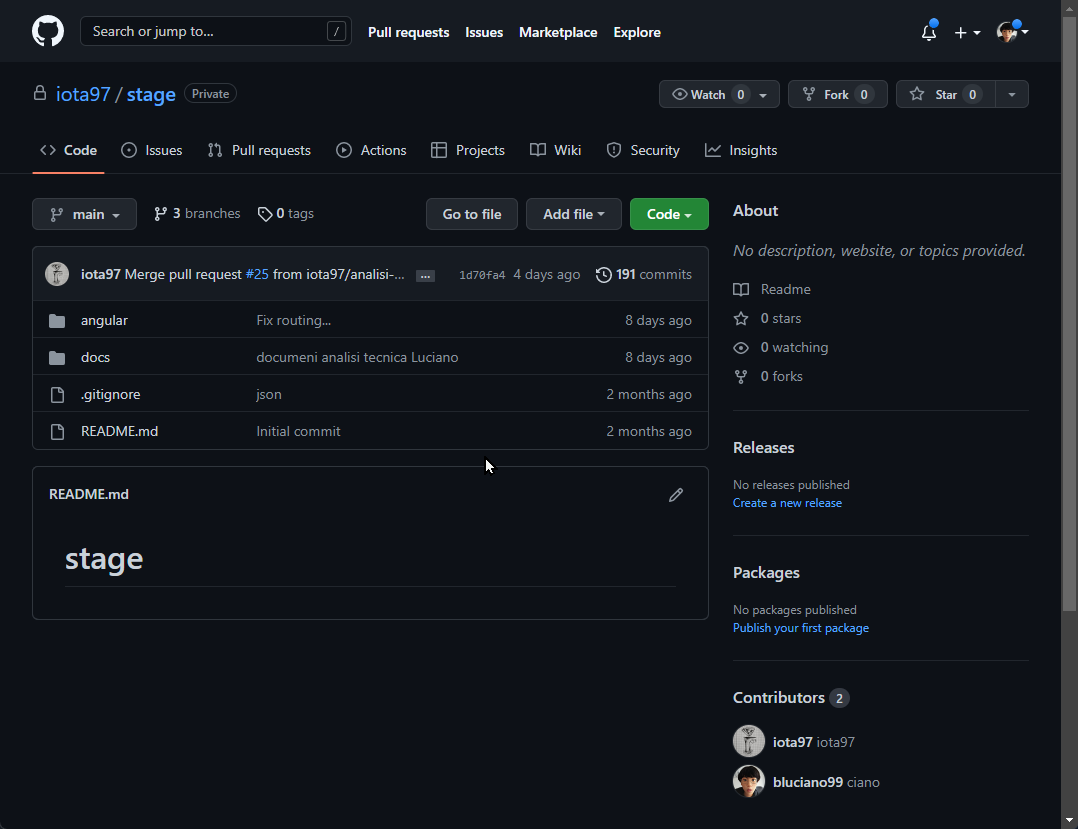
\includegraphics[scale=0.45]{github.png}
    \caption{Repo su GitHub per il progetto sushi-lab}
\end{figure}
\subsubsection{Visual Studio Code:}
Un editor sviluppato da Microsoft. Contiene tutte le funzionalità di un editor ed è completamente gratuita. Le principali funzionalità utilizzate per il progetto sono:
\begin{itemize}
    \item Le estensioni per il codice html, css e TypeScript;
    \item Il source control di Git integrato con Visual Studio Code;
    \item La funzione search con la quale è possibile ricercare un termine dentro tutti i file e fare la sostituzione velocemente.
\end{itemize}
\begin{figure}[H]
    \centering
    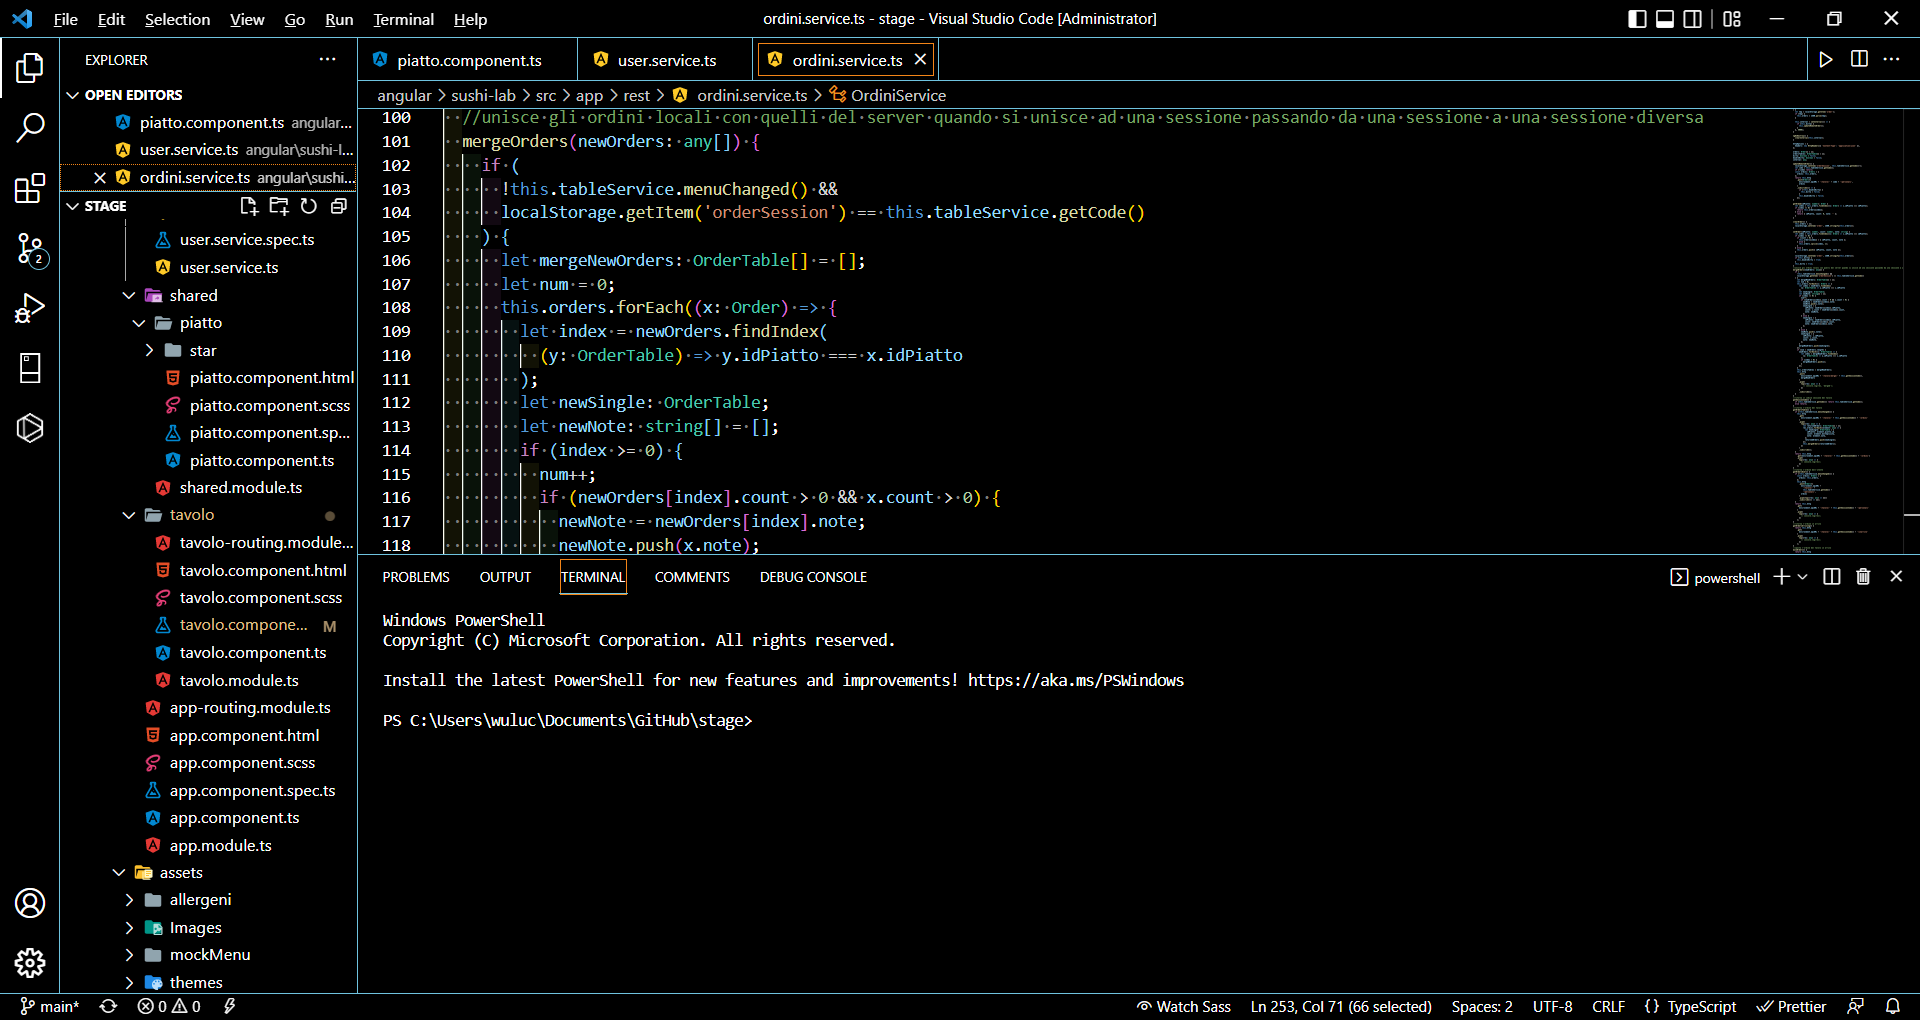
\includegraphics[scale=0.35]{vscode.png}
    \caption{Interfaccia di Visual Studio Code}
\end{figure}
\subsubsection{Google Chrome:}
Un browser web sviluppato da Google. È il browser più popolare nel mondo grazie alla sua buona stabilità ed elevata velocità. La maggiore funzionalità utilizzata di Chrome durante lo sviluppo è lo strumento ispeziona, che permette di vedere tutti i dati di uno specifico elemento HTML presente nella pagina, in più è possibile vedere tutti i dati salvati in locale della pagina.
\begin{figure}[H]
    \centering
    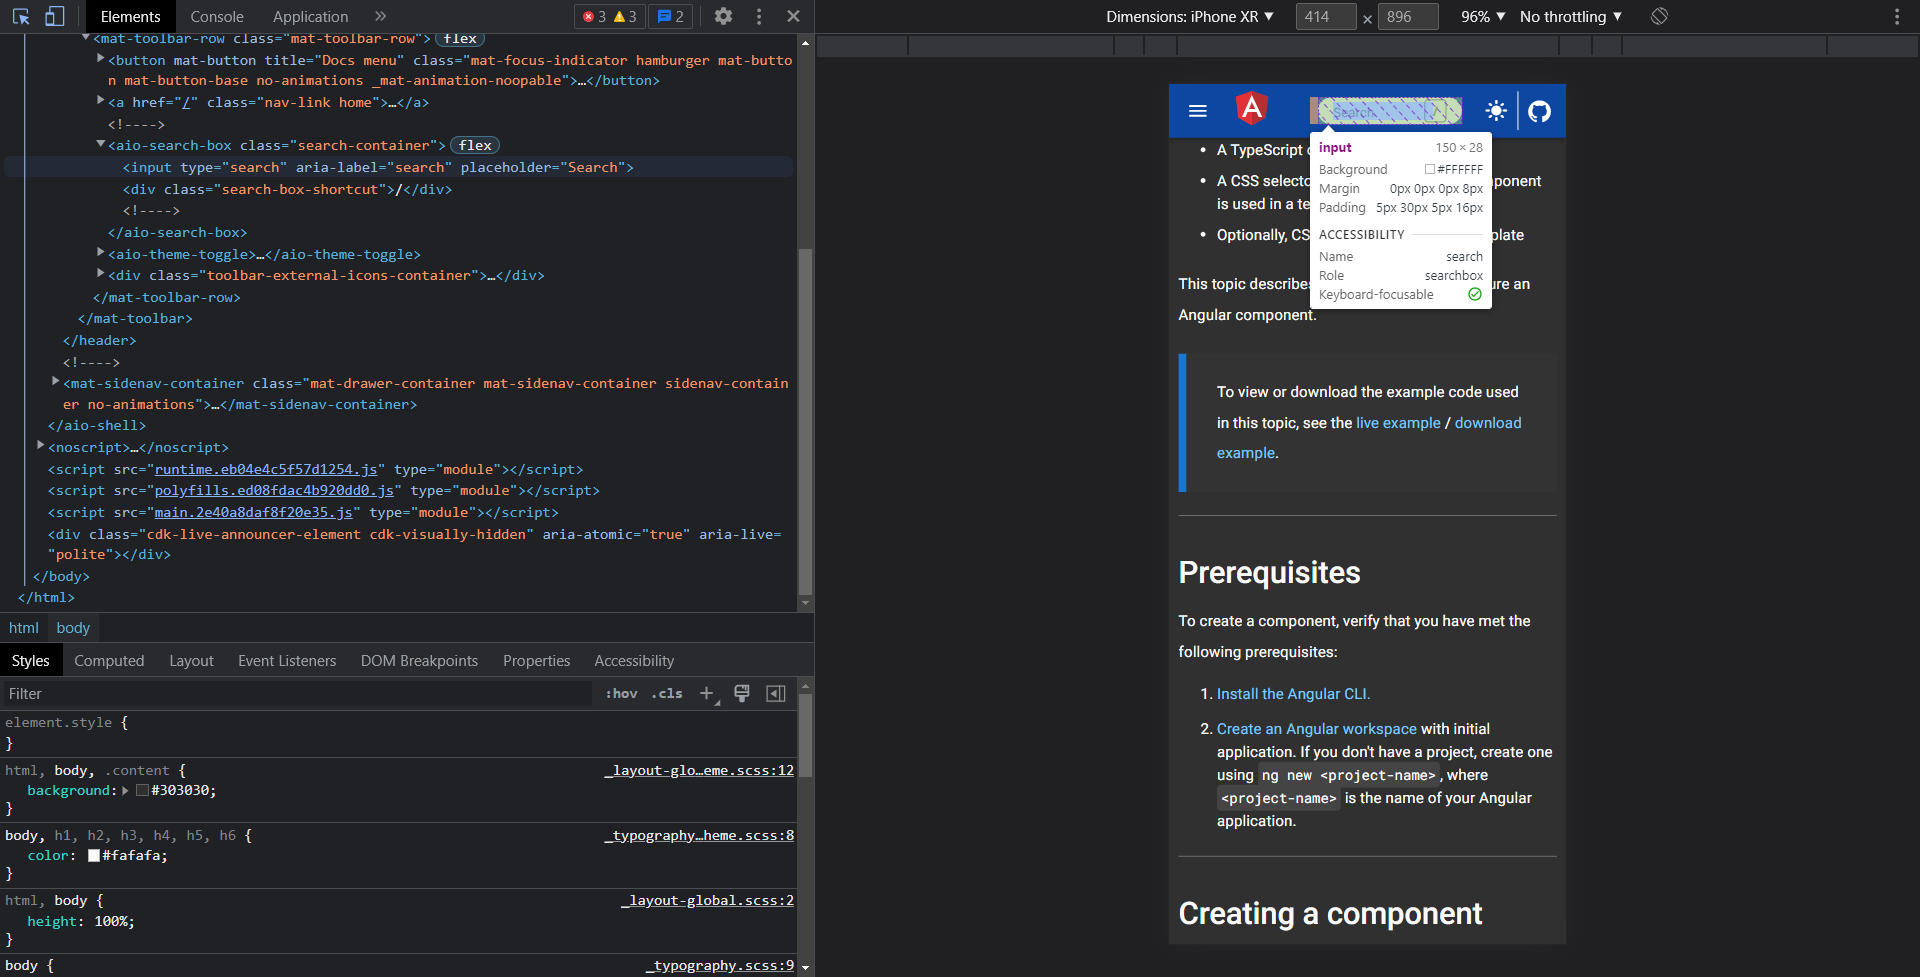
\includegraphics[scale=0.3]{chrome.png}
    \caption{Interfaccia con lo strumento ispeziona di Goolge Chrome}
\end{figure}
% \begin{center}
    
%     \begin{tabular}{ |p{3cm}|p{3cm}|p{3cm}|  }
%         \hline
%         \multicolumn{3}{|c|}{Country List} \\
%         \hline
%         Country Name or Area Name& ISO ALPHA 2 Code &ISO ALPHA 3 \\
%         \hline
%         Afghanistan & AF &AFG \\
%         Aland Islands & AX   & ALA \\
%         Albania &AL & ALB \\
%         Algeria    &DZ & DZA \\
%         American Samoa & AS & ASM \\
% Andorra & AD & AND   \\
% Angola & AO & AGO \\
% \hline
% \end{tabular}
% \end{center}